\documentclass[letterpaper,11pt]{article}
\usepackage[utf8]{inputenc} 
\usepackage{amsmath}
\usepackage{geometry}
\usepackage{graphicx}
\usepackage{tikz}
\usepackage{xcolor}
\usepackage{hyperref}
\usepackage{float} 
\usetikzlibrary{shapes.geometric, arrows, positioning}
\geometry{margin=1in}

\title{\textbf{Research Project}}
\author{} 
\date{\today}

\begin{document}

%\maketitle
%\tableofcontents

\newpage
\section*{Models}
\begin{flushright}
February 3, 2025
\end{flushright}
\hrule
\vspace{0.2in}

\begin{center}
    \subsection*{FFNN MLP}
    FeedFoward Neural network Multilayer Perceptron.
\end{center}
  
\begin{figure}[H]
    \centering
    \begin{minipage}[b]{0.45\textwidth}
      \centering
      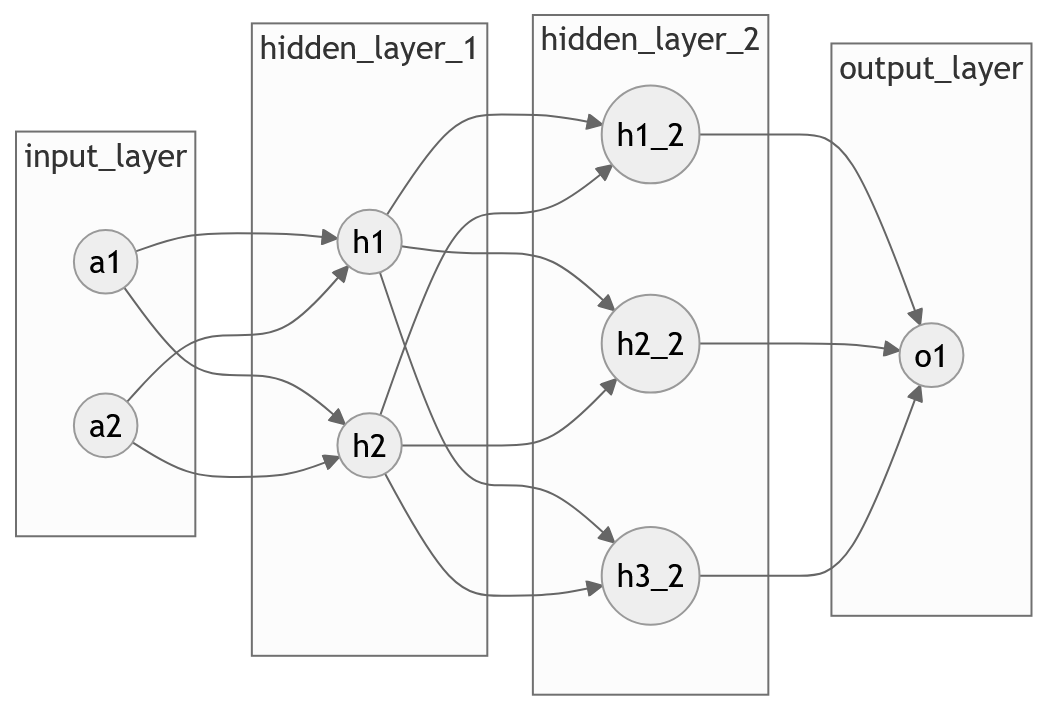
\includegraphics[width=\linewidth]{img/ffnn_exemple.png} 
    \end{minipage}
    \hfill
    \begin{minipage}[b]{0.45\textwidth}
      \centering
      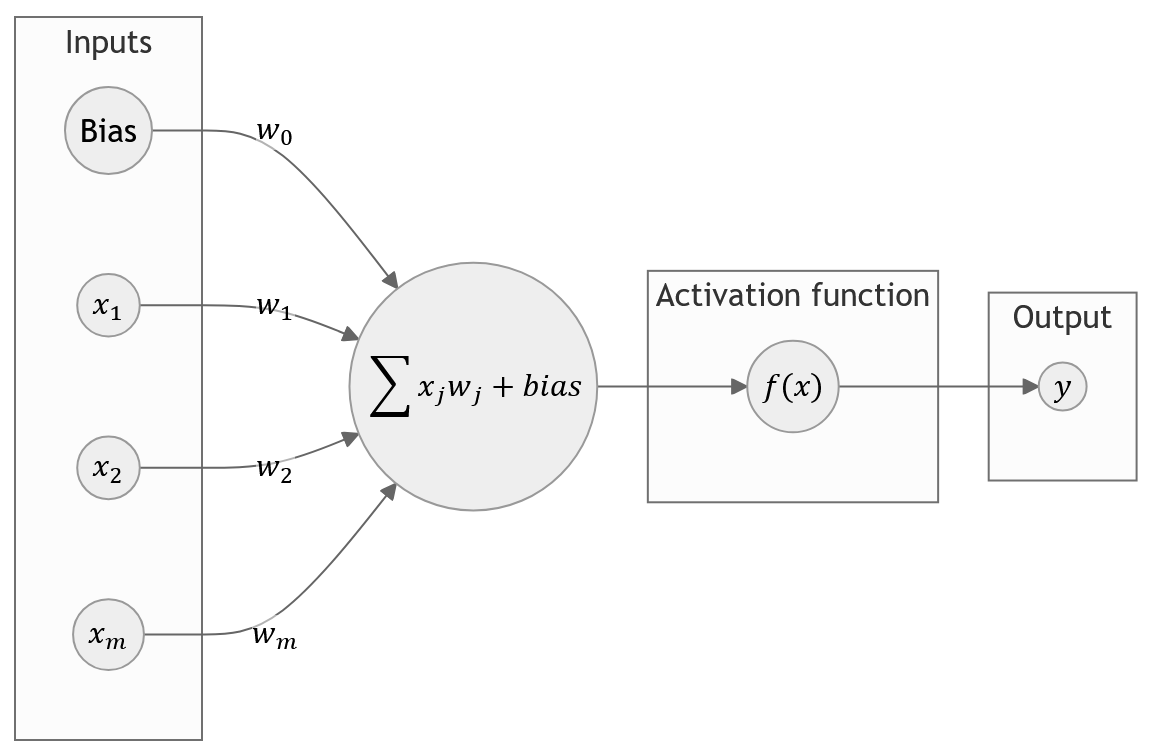
\includegraphics[width=\linewidth]{img/perceptron.png}
    \end{minipage}
  \end{figure}


Classical FeedFoward Neural network, multilayer perceptron.
The input vector :
\[
\mathbf{x} = [x_1, x_2, \ldots, x_n]
\]

Then on the first hidden layer, each perceptron follow :

\[
\mathbf{z} = \mathbf{W}\mathbf{x} + \mathbf{b}
\]

With an acivation function typicly sigmoid, ReLU, or tanh as :

\[
\mathbf{a} = \sigma(\mathbf{z})
\]


Until the output layers wich follow : 
\[
\mathbf{z}_{\text{out}} = \mathbf{W}_{\text{out}}\mathbf{a} + \mathbf{b}_{\text{out}}
\]

and same for the activation :

\[
\mathbf{y} = \sigma_{\text{out}}(\mathbf{z}_{\text{out}})
\]

The overall relationship between the input x and the output y can be viewed as a composite function of the linear transformations and activation functions applied at each layer. This can be expressed as:

\begin{align}
\mathbf{y} = \sigma_{\text{out}}(\mathbf{W}_{\text{out}} \sigma_L(\mathbf{W}_L \ldots \sigma_2(\mathbf{W}_2 \sigma_1(\mathbf{W}_1 \mathbf{x} + \mathbf{b}_1) + \mathbf{b}_2) \ldots + \mathbf{b}_L) + \mathbf{b}_{\text{out}})
\end{align}


\newpage
\begin{center}
    \subsection*{LSTM}
    Long Short Term Memory
\end{center}


\begin{figure}[H]
    \centering
    \begin{minipage}[b]{0.40\textwidth}
      \centering
      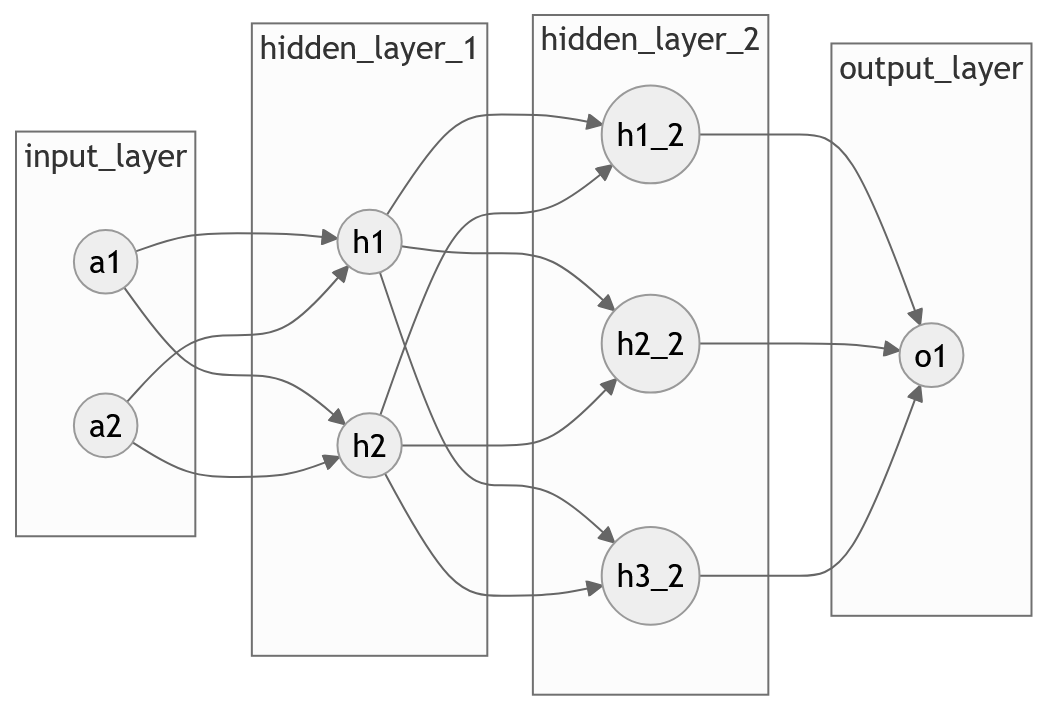
\includegraphics[width=\linewidth]{img/ffnn_exemple.png} 
    \end{minipage}
    \hfill
    \begin{minipage}[b]{0.49\textwidth}
      \centering
      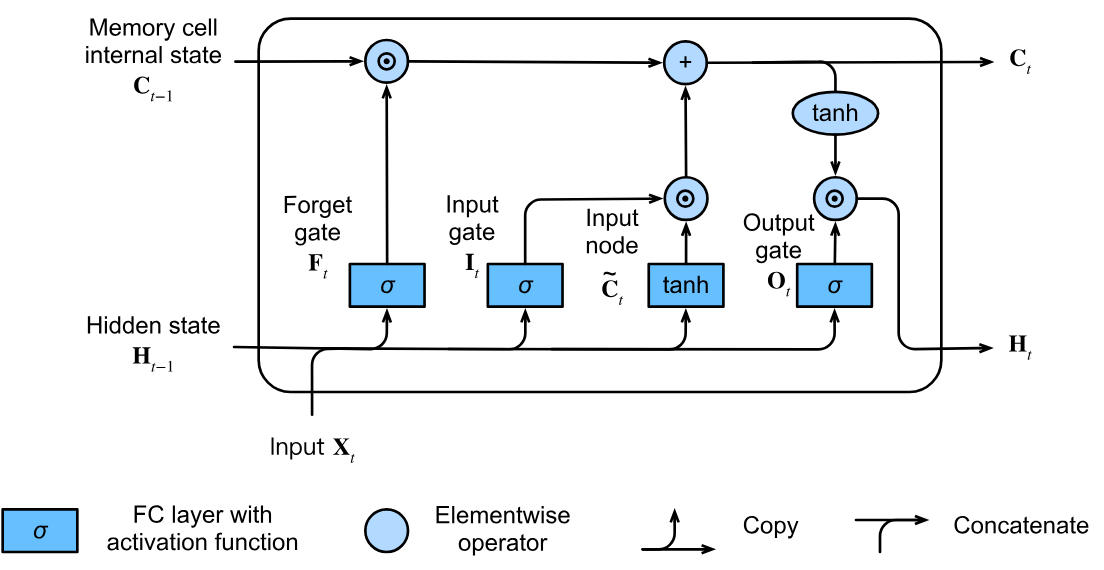
\includegraphics[width=\linewidth]{img/lstm.png}
    \end{minipage}
  \end{figure}


  Long Short-Term Memory (LSTM) network is a type of recurrent neural network (RNN) designed for sequential data, such as time series or natural language. LSTMs have memory cells and gates, allowing them to capture and retain dependencies over long sequences.\\

 Each LSTM cell consists of a cell state and three types of gates: the \textbf{forget} gate, \textbf{input} gate, and \textbf{output} gate.
 \begin{enumerate}
    \item The forget gate decides which information from the previous cell state to discard
    \item the input gate determines what new information to store in the cell state
    \item and the output gate controls what information to pass to the next hidden state
 \end{enumerate}

\bigskip


At each time step \( t \), the LSTM receives an input vector \(\mathbf{x}_t\) and the previous hidden state \(\mathbf{h}_{t-1}\).


\paragraph*{Forget Gate}
Decides what information to discard from the previous cell state:
\[
\mathbf{F}_t = \sigma(\mathbf{W}_f \cdot [\mathbf{H}_{t-1}, \mathbf{X}_t] + \mathbf{b}_f)
\]

\paragraph*{Input Gate}
Decides what new information to store in the cell state:
\[
\mathbf{I}_t = \sigma(\mathbf{W}_i \cdot [\mathbf{H}_{t-1}, \mathbf{X}_t] + \mathbf{b}_i)
\]

\paragraph*{Output Gate}
Decides what information to output based on the cell state:
\[
\mathbf{O}_t = \sigma(\mathbf{W}_o \cdot [\mathbf{H}_{t-1}, \mathbf{X}_t] + \mathbf{b}_o)
\]

\paragraph*{Candidate Cell State}
Generates new candidate values to add to the cell state:
\[
\tilde{\mathbf{C}}_t = \tanh(\mathbf{W}_C \cdot [\mathbf{H}_{t-1}, \mathbf{X}_t] + \mathbf{b}_c)
\]

\paragraph*{Cell State Update}
Updates the cell state using the forget and input gates:
\[
\mathbf{C}_t = \mathbf{F}_t \odot \mathbf{C}_{t-1} + \mathbf{I}_t \odot \tilde{\mathbf{C}}_t
\]


\paragraph*{Hidden State Update (Output)\\}
Updates the hidden state using the output gate and the updated cell state:
\[
\mathbf{H}_t = \mathbf{O}_t \odot \tanh(\mathbf{C}_t)
\]

Or we can rewrite :

\begin{align}
    \mathbf{H}_t = & \sigma(\mathbf{W}_o \cdot [\mathbf{H}_{t-1}, \mathbf{X}_t] + \mathbf{b}_o) \nonumber \\
    & \odot \tanh\Bigl(\sigma(\mathbf{W}_f \cdot [\mathbf{H}_{t-1}, \mathbf{X}_t] + \mathbf{b}_f) \odot \mathbf{C}_{t-1} \nonumber \\
    & + \sigma(\mathbf{W}_i \cdot [\mathbf{H}_{t-1}, \mathbf{X}_t] + \mathbf{b}_i) \odot \tanh(\mathbf{W}_C \cdot [\mathbf{H}_{t-1}, \mathbf{X}_t] + \mathbf{b}_c)\Bigr)
\end{align}



    

\paragraph*{Output}
The output of the LSTM at time step \( t \) is the hidden state \(\mathbf{H}_t\). For a sequence of inputs, the final output can be based on the hidden state at the last time step or a function of all hidden states.






%\subsection*{Transformers}


\newpage
\begin{center}
    \subsection*{Volatility model parameters}
\end{center}

\begin{minipage}[t]{0.49\textwidth}
    \textbf{Inputs (Features) :}
    \begin{enumerate}
        \item Inflation
        \item CPI
        \item Treasury\_Yield
        \item Open
        \item High
        \item Low
        \item Close
        \item SP\_Adj\_Close
        \item Volume
        \item GDP
        \item mortage
        \item unemployement
        \item def\_fund\_rate
        \item Volatility(current)
        \item returns
        \item EWMA\_VM
        \item GARCH\_VM
        \item EGARCH\_VM
        \item RagerSatchell\_VM
        \item garman\_klass
        \item parkison
        \item yang\_zhang
    \end{enumerate}
\end{minipage}
\hfill
\begin{minipage}[t]{0.49\textwidth}
    \textbf{Output (Target) :}
    \begin{enumerate}
        \item volatility\_forcast
    \end{enumerate}
    %\vspace{0.5in}
    %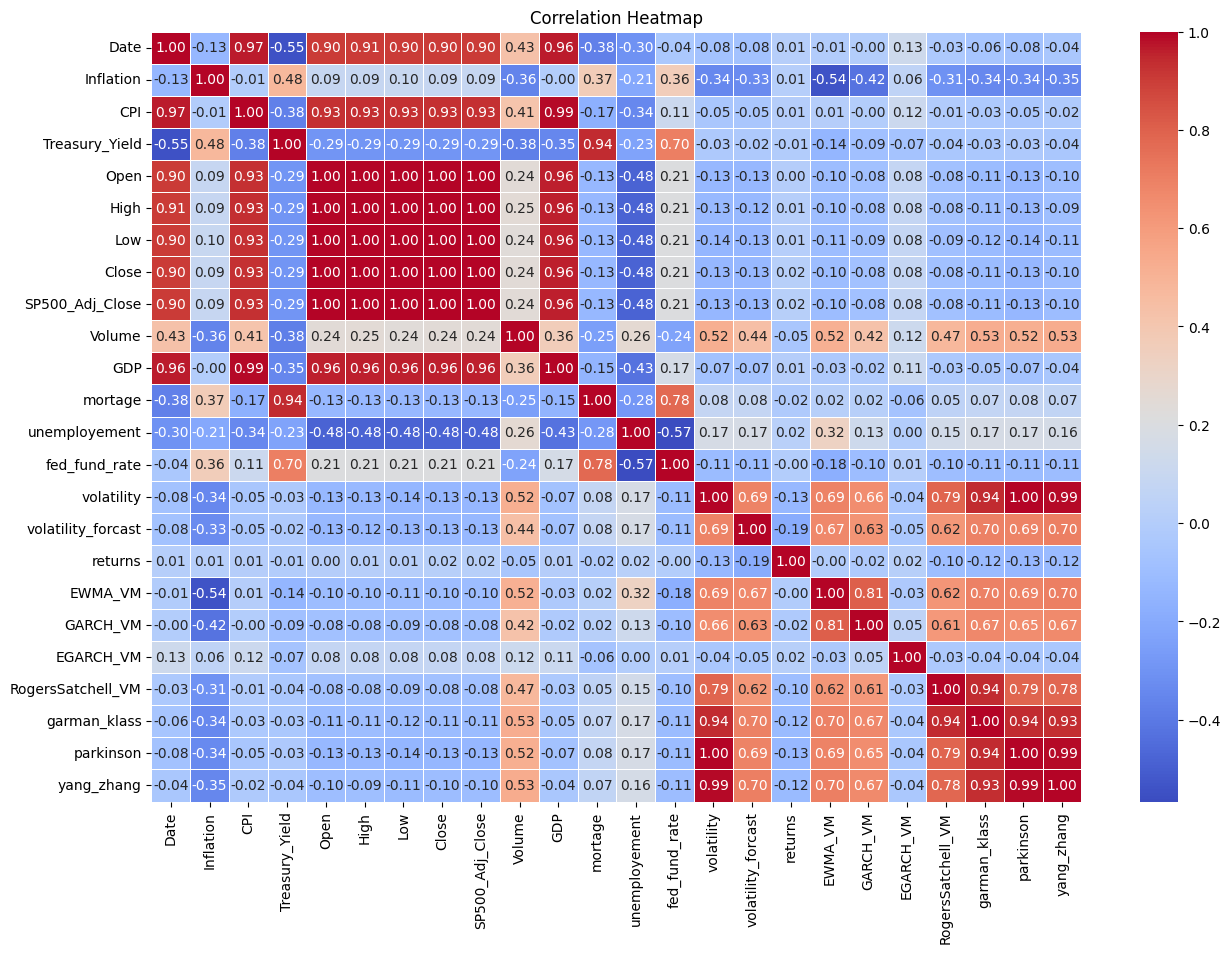
\includegraphics[width=\linewidth]{img/corr_matrix.png}

\end{minipage}


\newpage
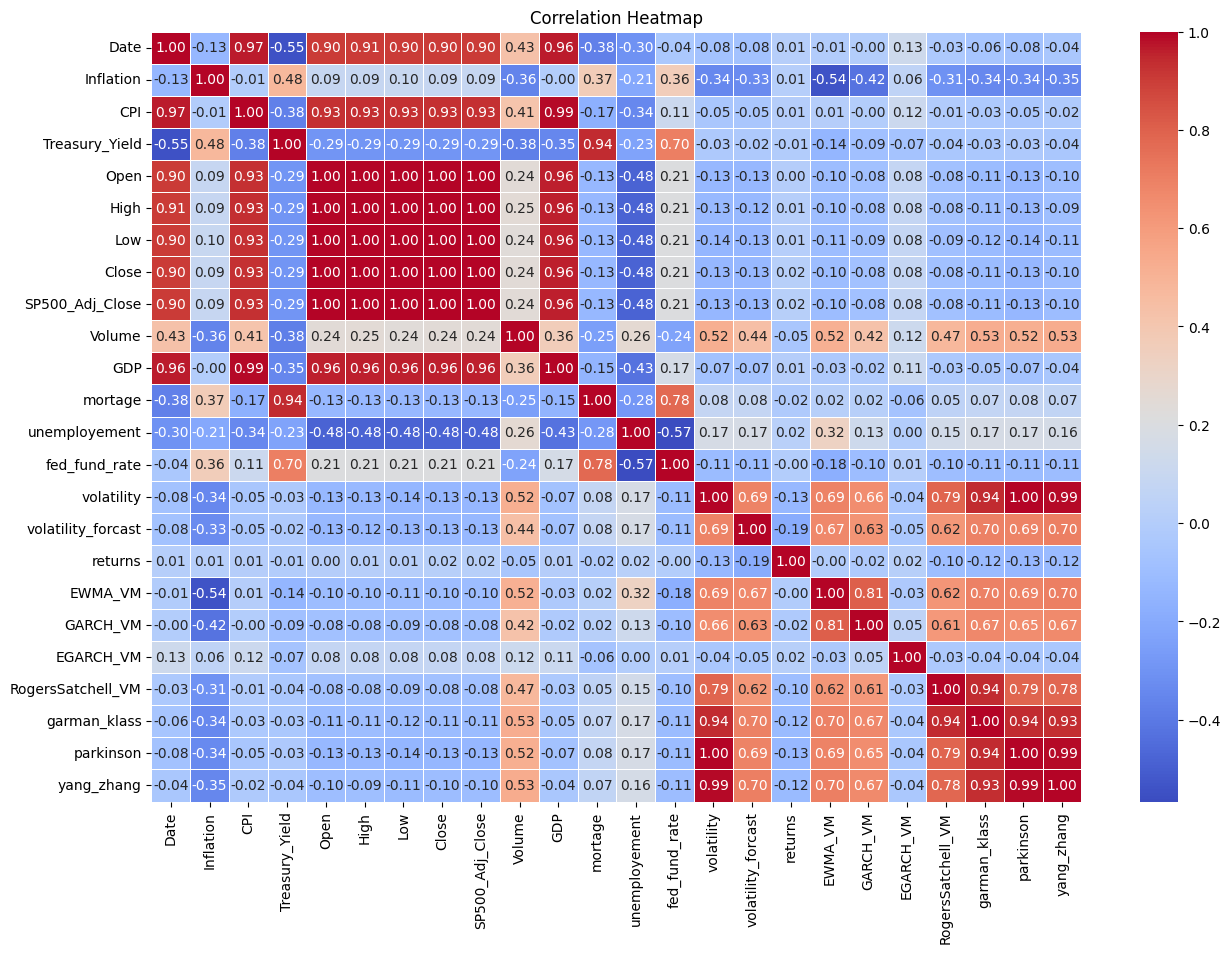
\includegraphics[width=\linewidth]{img/corr_matrix.png}





\end{document}
